\documentclass[12pt]{article}
%Gummi|065|=)
\usepackage{amsmath, amsfonts, amssymb}
\usepackage[margin=0.5in]{geometry}
\usepackage{xcolor}
\usepackage{graphicx}

\newcommand{\off}[1]{}
\DeclareMathSizes{20}{30}{20}{18}

\newcommand{\two }{\sqrt[3]{2}}
\newcommand{\four}{\sqrt[3]{4}}


\usepackage{tikz}

\title{Nilsequences}
\author{John D Mangual}
\date{}
\begin{document}

\fontfamily{qag}\selectfont \fontsize{12.5}{15}\selectfont

\maketitle

\noindent Terence Tao sees a lot of things, but he writes in an obfuscated way, and I think he misses a lot of things.  About 10 years ago, I was introduced to the topic of \textbf{nilsequences} in a course of Dynamics and Number Theory.  I did nothing with it.  Let's read Terry's latest blog on this topic\footnote{\texttt{https://terrytao.wordpress.com/2017/04/28/notes-on-nilcharacters-and-their-symbols/}}. \\ \\
Part of it is like\dots where do fractions come from?  \\ \\
If we take scientific measurement, there's quite a bit error that obstructs us from observing the most delicate patterns.  In fact, shielding us completely from finding them (or protecting us). \\ \\
$\sqrt{2} = 1.414213562373095048801688724209698078
5696718753769480731766797379907324784621070388503 $ \\ \\
If you examine the digits carefully\footnote{\texttt{http://www.gutenberg.org/files/129/129.txt}} we can prove the decimals do not exhibit any pattern in the decimal expension.  However, if we use continued fractions: \\ \\
$\sqrt{2} = [1; 2,2,2,2,2 , \dots ] $
and this is a nicer system since we have exponential convergence of the the number.  Here the error is $10^{-6}$ (microscopic). \\ \\
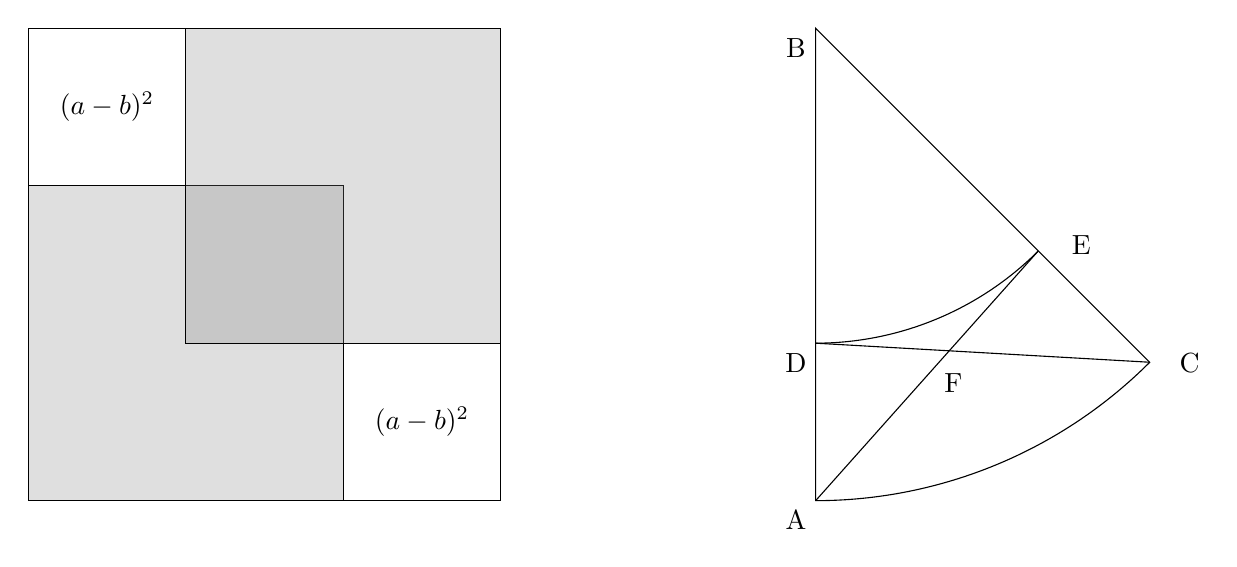
\begin{tikzpicture}

\begin{scope}
\draw (0,0)--(6,0)--(6,6)--(0,6)--cycle;
\draw[opacity=0.25, fill=black!50!white] (0,0)--(4,0)--(4,4)--(0,4)--cycle;
\draw (0,0)--(4,0)--(4,4)--(0,4)--cycle;
\draw[opacity=0.25, fill=black!50!white] (2,2)--(6,2)--(6,6)--(2,6)--cycle;
\draw (2,2)--(6,2)--(6,6)--(2,6)--cycle;
\node at (1,5) {$(a-b)^2$};
\node at (5,1) {$(a-b)^2$};
\end{scope}

\begin{scope}[xshift=10cm]

\draw (0,6)--(0,0)--(0,0) arc (90:135:-6)--cycle;
\draw (0,2) arc (90:135:-4);
\node at (-0.25,-0.25) {A};
\node at (-0.25,-0.25+6) {B};
\node at (-0.25+5,-0.25+2) {C};
\node at (-0.25,-0.25+2) {D};
\node at (-0.25+3.625,-0.25+3.5) {E};
\node at (-0.25+2,-0.25+1.75) {F};
\draw (0,2)--(6*1.414/2, 6 - 6*1.414/2);
\draw (0,0)--(4*1.414/2, 6 - 4*1.414/2);

\end{scope}

\end{tikzpicture} \\
These pictures lead to two different proofs that $\sqrt{2} \notin \mathbb{Q}$.  They are both geometric proofs, and argue by infinite descent.  Therefore, there must have been an \`{e}tale cohomology. \\ \\
I have no idea what \`{e}tale cohomology and the books do not simplify it enough for me. \\ 
Forget it.  One way to get meaningful numbers to arbitrary accuracy is to observe a dynamical system over time and take detailed measurements.  And you will see.

\newpage

\vfill


\noindent Here's a reading list. I will leave in the Class Field Theory book since even though don't need it any way (we are solving over $\mathbb{Z}$), in fact we may need it anyway.

\begin{thebibliography}{}

\item Nancy Childress \textbf{Class Field Theory} (Universitext).  Spinger, 2009.

\item Ben Green, Terence Tao, Tamar Ziegler. \textbf{An inverse theorem for the Gowers $U^{s+1}[N]$-norm} \texttt{arXiv:1009.3998}

\item Ben Green \textbf{Approximate algebraic structure} \texttt{arXiv:1404.0093}

\end{thebibliography}

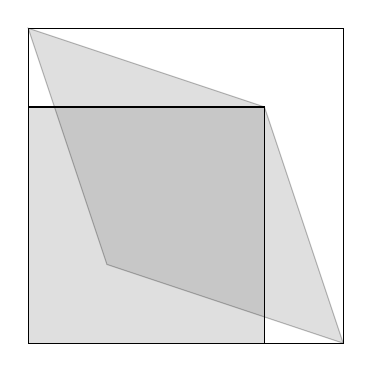
\begin{tikzpicture}
\draw (0,0)--(4,0)--(4,4)--(0,4)--cycle;
\draw[opacity=0.25, fill=black!50!white] (0,0)--(3,0)--(3,3)--(0,3)--cycle;
\draw (0,0)--(3,0)--(3,3)--(0,3)--cycle;
\draw[opacity=0.25, fill=black!50!white] (1,1)--(4,0)--(3,3)--(0,4)--cycle;
\draw (0,0)--(3,0)--(3,3)--(0,3)--cycle;
\end{tikzpicture}

\end{document}